% Inserir no capítulo de experimentos da dissertação.
% Requer: \usepackage{booktabs} e \usepackage{graphicx}

\section{Piloto condicional com o canal infravermelho C13 do GOES-16}
\label{sec:piloto-goes-c13-condicional}

Esta seção apresenta um piloto exploratório para investigar se a temperatura de brilho do canal infravermelho C13 do satélite GOES-16 contém informação complementar ao produto visual do radar do Sumaré. O objetivo não é avaliar ainda um modelo operacional de nowcasting, mas responder à seguinte questão: quando há sinais de radar visualmente comparáveis na vizinhança das estações, o C13 ajuda a distinguir casos com chuva futura de casos sem chuva?

O C13 é um canal infravermelho térmico. Seu valor representa aproximadamente a temperatura de brilho do topo da nuvem ou da superfície observada pelo satélite, em kelvin. Valores menores tendem a estar associados a topos de nuvens mais frios e altos. Essa relação é meteorologicamente relevante para convecção, mas C13 não mede precipitação diretamente e não substitui o radar ou os pluviômetros.

\subsection{Seleção de pares condicionais}
\label{subsec:selecao-pares-c13}

Foram considerados 46.280 instantes elegíveis dos anos de 2023 e 2024. Cada instante elegível possui cinco janelas passadas de radar, cinco horizontes futuros e observações válidas das estações do AlertaRio. Para cada candidato, foram usados cinco frames de entrada, separados por 15 minutos, correspondentes aos instantes $T-75$, $T-60$, $T-45$, $T-30$ e $T-15$ minutos.

Um evento foi classificado como \textit{wet} quando a maior observação entre as estações no primeiro horizonte futuro ($T$) foi igual ou superior a 1,25~mm/15~min. Um controle seco foi definido de forma mais restritiva: todas as estações deveriam registrar 0,0~mm/15~min em cada um dos cinco horizontes futuros, de $T$ até $T+60$ minutos.

Para controlar aproximadamente a evidência disponível no radar, foi calculada, no último frame de entrada ($T-15$), a fração média de pixels RGB não pretos em uma vizinhança de raio dois pixels ao redor das 33 estações. Essa variável é denominada neste trabalho de \emph{fração de eco RGB}. Ela é apenas um indicador de presença visual de eco no produto de imagem; não é uma estimativa quantitativa de refletividade.

Os eventos \textit{wet} e os controles secos foram então pareados quando satisfaziam simultaneamente os seguintes critérios: mesmo ano, mesmo mês, mesma hora UTC, diferença máxima de 0,05 na fração de eco RGB e separação temporal mínima de 24 horas entre eventos selecionados. Foram obtidos 24 pares, totalizando 48 eventos. Um controle seco não apresentou nenhuma cena C13 causalmente disponível e foi excluído das métricas finais; a análise foi realizada, portanto, com 47 eventos.

\subsection{Aquisição causal do GOES-16}
\label{subsec:aquisicao-causal-goes}

Para cada um dos cinco instantes de entrada, a versão V1 do piloto selecionou a cena C13 mais recente cujo instante de início fosse anterior ou igual ao instante correspondente do radar. As cenas Full Disk foram baixadas temporariamente, reprojetadas para a mesma grade de $128 \times 128$ pixels do radar e removidas após o processamento. A auditoria verificou zero violações dessa condição baseada no início da cena.

Essa convenção V1 é suficiente para o objetivo exploratório do piloto, mas não garante causalidade estrita por pixel: uma varredura Full Disk pode terminar após o instante do radar. Por esse motivo, a Seção~\ref{sec:smoke-goes16-c13} introduz o contrato V2, que exige que o fim da cena seja anterior ou igual ao início da janela de radar antes de qualquer geração histórica destinada ao treinamento.

Embora cinco frames C13 tenham sido armazenados e inspecionados visualmente para cada evento, a análise quantitativa descrita a seguir usa, nesta primeira versão, apenas atributos do último frame disponível em $T-15$. Essa escolha reduz a complexidade do piloto e deixa explícito que a dinâmica temporal completa do satélite ainda não foi explorada pelo classificador.

\subsection{Features e classificador}
\label{subsec:features-classificador-c13}

As observações das 33 estações foram agregadas para produzir um único vetor de atributos por evento. Portanto, as estações não foram tratadas como exemplos independentes, evitando inflar artificialmente o tamanho amostral. Foram comparados dois classificadores de regressão logística:

\begin{itemize}
    \item \textbf{Radar RGB}: média e máximo da fração de eco RGB nas vizinhanças das estações;
    \item \textbf{Radar RGB + C13}: os dois atributos do radar, acrescidos da média e do mínimo da temperatura C13 nas vizinhanças das estações.
\end{itemize}

A regressão logística é um classificador linear probabilístico que estima a probabilidade de um evento pertencer à classe \textit{wet}. Ela foi escolhida por sua simplicidade e interpretabilidade: o objetivo do piloto é avaliar a informação disponível nas fontes, não otimizar uma arquitetura profunda.

A avaliação foi realizada por validação cruzada estratificada em cinco folds. Foi usado o agrupamento por \texttt{pair\_id}: os dois elementos de cada par, o evento chuvoso e o controle seco correspondente, permaneceram sempre no mesmo fold. Dessa forma, o classificador não foi treinado em um membro do par e avaliado no outro.

\subsection{Resultados}
\label{subsec:resultados-piloto-c13}

A Tabela~\ref{tab:piloto-c13-condicional} apresenta as métricas fora da amostra obtidas na validação cruzada. A área sob a curva ROC (AUC) mede a capacidade de ordenar eventos chuvosos acima dos controles secos. A \emph{average precision} resume o desempenho na recuperação de eventos positivos.

\begin{table}[htbp]
\centering
\caption{Desempenho fora da amostra no piloto condicional por pares.}
\label{tab:piloto-c13-condicional}
\begin{tabular}{lrr}
\toprule
\textbf{Modelo} & \textbf{AUC ROC} & \textbf{Average Precision} \\
\midrule
Radar RGB & 0,800 & 0,785 \\
Radar RGB + C13 & 0,868 & 0,817 \\
\bottomrule
\end{tabular}
\end{table}

As Figuras~\ref{fig:goes-c13-pair-wet} e \ref{fig:goes-c13-pair-dry} apresentam um par condicionado representativo. Os dois casos possuem a mesma fração média de eco RGB na vizinhança das estações (0,00485), mas têm desfechos distintos. A primeira linha de cada figura mostra C13 do GOES-16; a segunda mostra o produto RGB do radar. Os círculos brancos indicam as estações e seu tamanho é proporcional à chuva observada no horizonte futuro.

\begin{figure}[htbp]
\centering
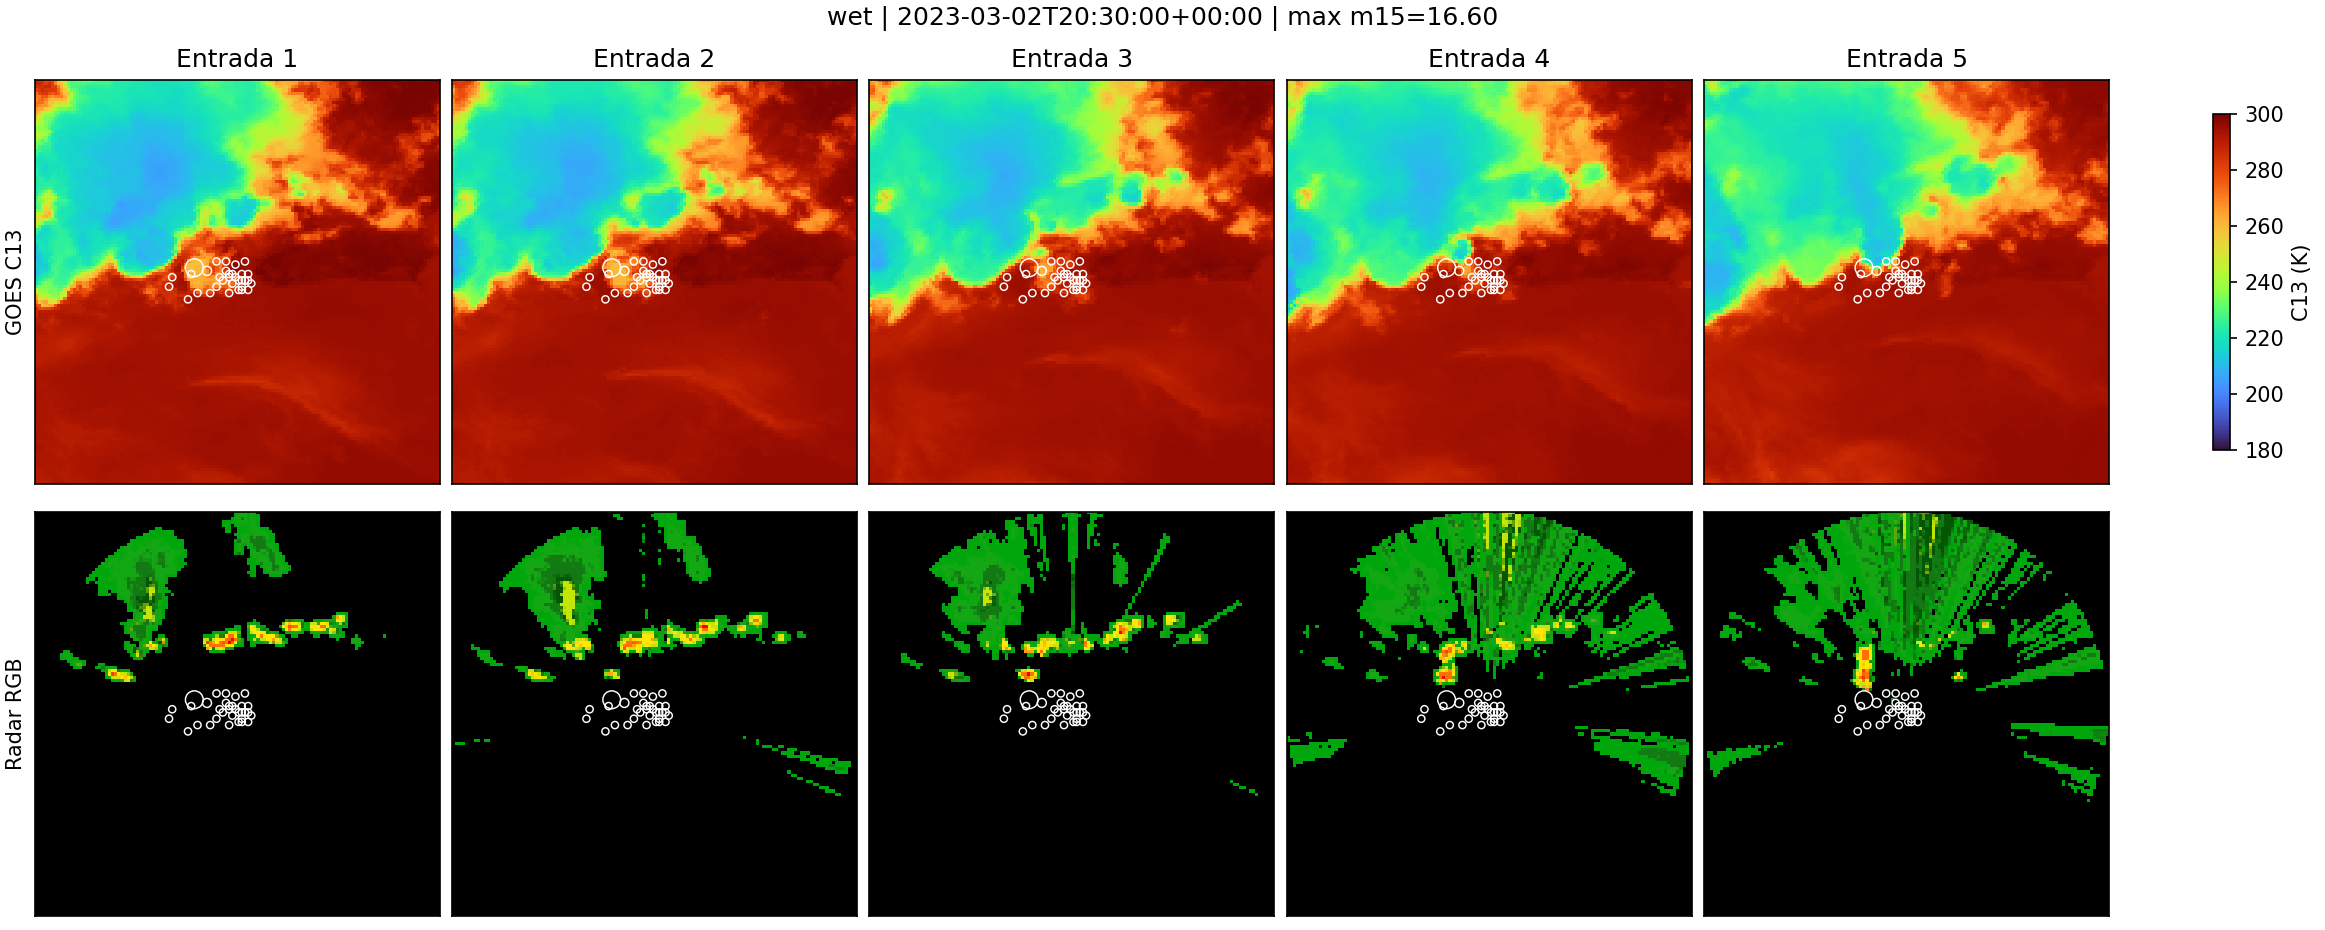
\includegraphics[width=\textwidth]{figures/goes16_hard_pair_014_wet.png}
\caption[Par condicionado com chuva observada.]{Par condicionado com chuva observada em 2 de março de 2023. Os cinco painéis correspondem às entradas entre $T-75$ e $T-15$ minutos; a máxima precipitação observada no horizonte futuro foi 16,6~mm/15~min. Embora o proxy de eco RGB local seja baixo, a região das estações se aproxima de uma área de C13 mais frio ao longo da sequência. A figura ilustra uma situação em que o sinal infravermelho pode complementar a evidência local limitada do radar RGB.}
\label{fig:goes-c13-pair-wet}
\end{figure}

\begin{figure}[htbp]
\centering
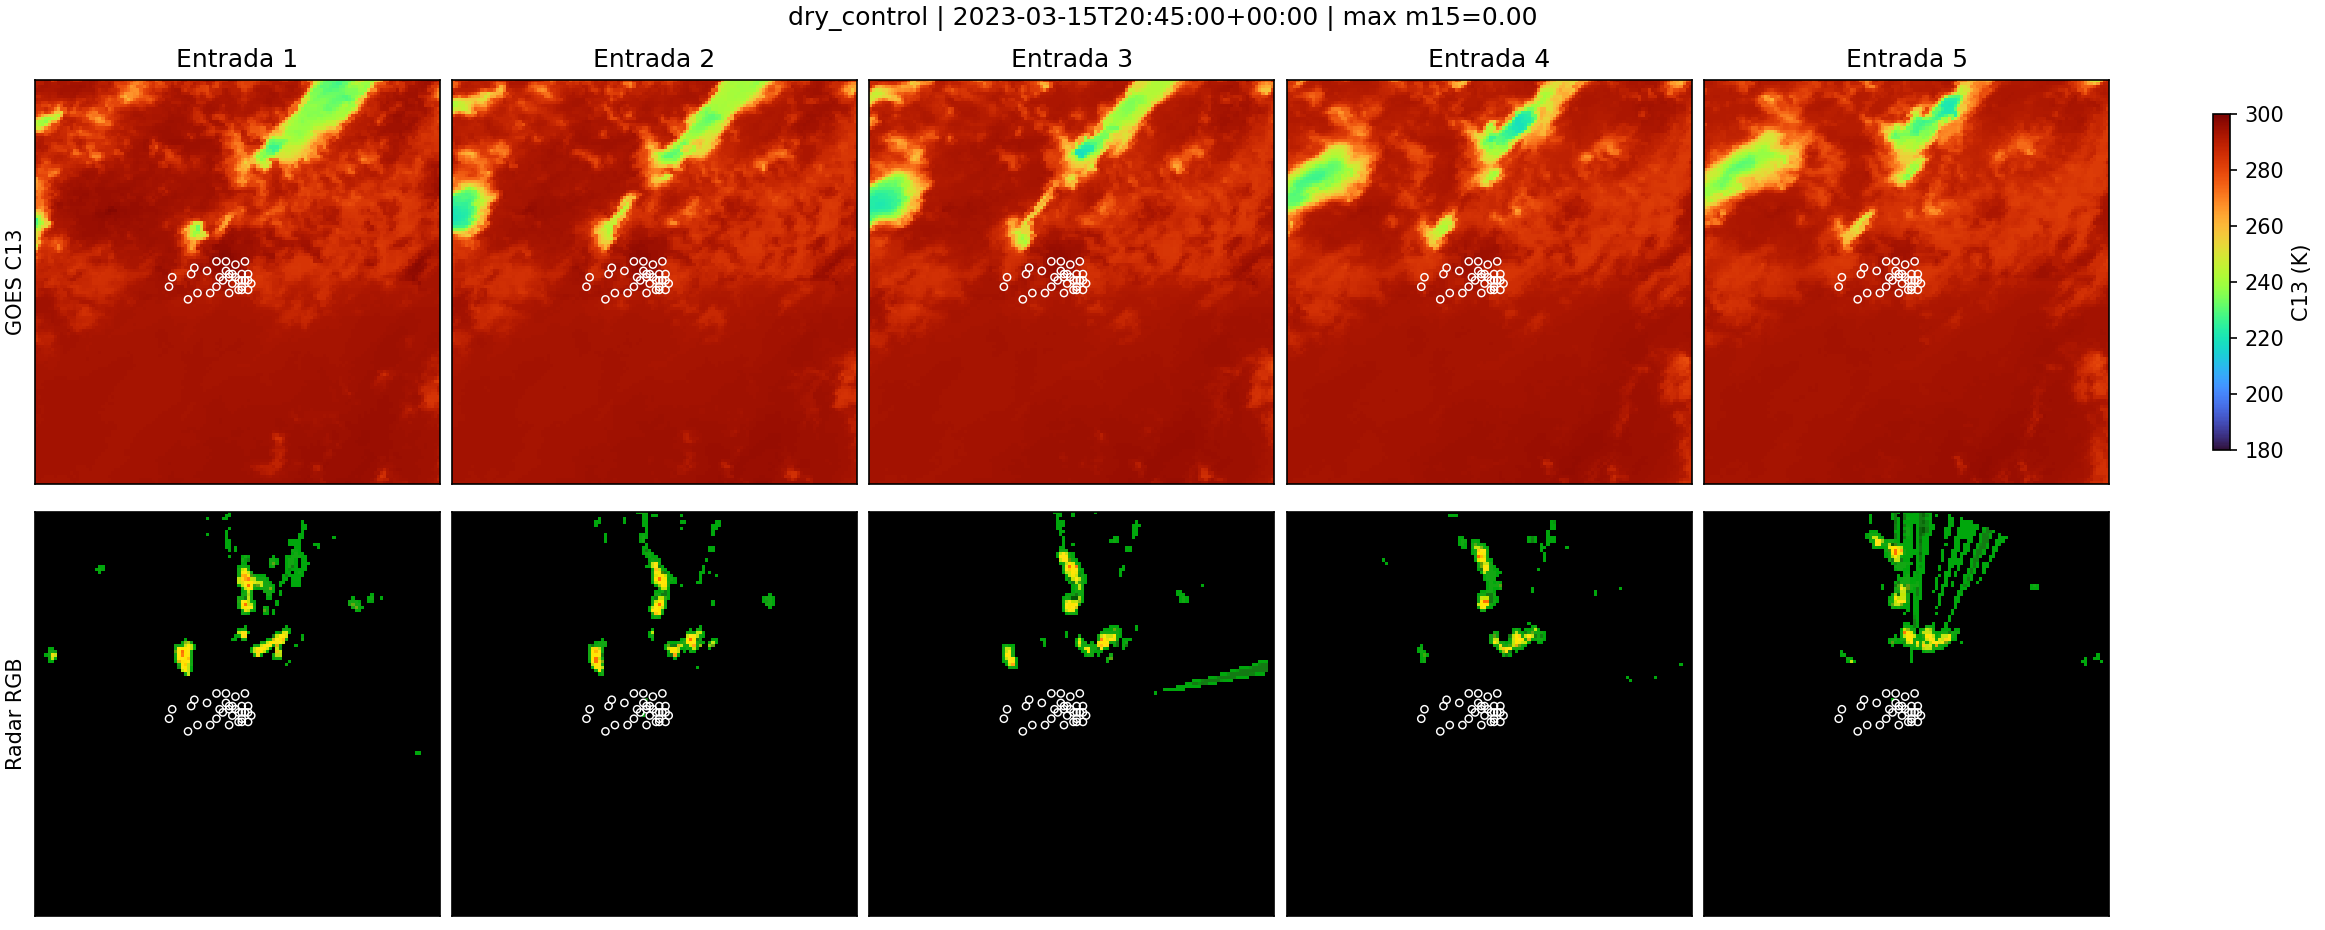
\includegraphics[width=\textwidth]{figures/goes16_hard_pair_014_dry.png}
\caption[Controle seco do par condicionado.]{Controle seco pareado, em 15 de março de 2023. Os cinco horizontes futuros registraram 0,0~mm/15~min em todas as estações. A fração média de eco RGB local é a mesma do evento chuvoso da Figura~\ref{fig:goes-c13-pair-wet}, mas o campo C13 sobre as estações é predominantemente mais quente. A comparação evidencia que a temperatura do topo de nuvem pode acrescentar informação em condições de eco de radar semelhante.}
\label{fig:goes-c13-pair-dry}
\end{figure}

A adição de C13 elevou a AUC em 0,068 e a \emph{average precision} em 0,032. Diferentemente do piloto inicial, há sobreposição suficiente de eco de radar entre as classes: considerando a faixa de fração de eco RGB menor ou igual a 0,05, permaneceram 38 eventos, dos quais 16 chuvosos e 22 controles secos. Assim, o resultado é consistente com a hipótese de que C13 oferece informação complementar em situações nas quais a presença de eco no radar é fraca ou ambígua.

Também há coerência física no sinal observado. A temperatura C13 média nas vizinhanças das estações foi 243,8~K nos eventos chuvosos e 275,3~K nos controles secos. A correlação de Spearman entre a variável ``frieza'' ($-$C13) e a chuva observada foi 0,268. Esses números indicam associação moderada, mas não determinística, entre nuvens frias e precipitação em superfície.

\subsection{Limitações e próximos passos}
\label{subsec:limitacoes-piloto-c13}

Os resultados devem ser interpretados como evidência de viabilidade, e não como demonstração de ganho preditivo operacional. A seleção dos eventos utilizou observações futuras para definir as classes e os pares; por isso, ela não reproduz o fluxo de inferência de um sistema em tempo real. Além disso, a amostra é pequena, contém apenas um canal do GOES-16, utiliza atributos resumidos do último frame e não emprega uma rede de nowcasting.

Os próximos experimentos devem ampliar a avaliação para uma divisão cronológica independente, usar a sequência temporal completa de C13 e comparar modelos multimodais que recebam radar, observações passadas das estações e satélite como entradas. A versão atual fornece uma justificativa técnica para essa expansão, mas não substitui a avaliação multianual rigorosa desses modelos.
